% \pdfpageattr {/Group << /S /Transparency /I true /CS /DeviceRGB>>}
\documentclass[10pt, xcolor={usenames, dvipsnames}]{beamer}

\usepackage[french, english]{babel}
\usepackage[utf8]{inputenc}
\usepackage[T1]{fontenc}
\usepackage{upgreek,textgreek}
\usepackage{animate}


\usepackage{changepage}

\usepackage{fnpct}

\usepackage{pifont}
\newcommand{\cmark}{\ding{51}}
\newcommand{\xmark}{\ding{55}}

\usepackage{amsmath}
\usepackage{amssymb}
\usepackage{bm}

\usepackage{graphicx}
\usepackage{hyperref}
\usepackage[style=alphabetic, autocite=inline, firstinits=true, maxnames=2]{biblatex}
\bibliography{bibliographie}
%\renewcommand*{\bibfont}{\small}

\usepackage{makecell}
\usepackage{tabularx, booktabs}
\usepackage{tikz}
\definecolor{light-gray}{gray}{0.65}
\tikzset{fade on/.code={\only<#1>{\color{light-gray}}}}
\tikzset{hide on/.code={\only<#1>{\color{white}}}}
\tikzset{bold on/.code={\only<#1>{\bfseries}}}
\tikzset{
  opinvisible/.style={opacity=0.2},
  visible on/.style={alt={#1{}{opinvisible}}},
  alt/.code args={<#1>#2#3}{%
    \alt<#1>{\pgfkeysalso{#2}}{\pgfkeysalso{#3}} % \pgfkeysalso doesn't change the path
  },
}

\usetikzlibrary{plotmarks,shapes,patterns}
\usepackage{colortbl}
\usepackage{ulem}
\usepackage{multicol}
\usepackage[overlay]{textpos}
\usepackage{multirow}
\usepackage{ragged2e}
\usepackage{rotating}
\usepackage{fancybox}
\usepackage{ulem}
\usepackage{overpic}
\usepackage{enumerate}
\usepackage{xfrac}
\usepackage{pgfplots}

\usepackage{transparent}

\usepackage{epstopdf}
\usepackage{epsfig}


\newcommand{\REF}{\textcolor{purple}{REF}}
\newcommand{\GO}[1]{\textcolor{blue}{#1}}
\newcommand{\YES}[1]{\textcolor{green}{#1}}
\newcommand{\NO}[1]{\textcolor{red}{#1}}

\newcommand{\BA}[1]{\textcolor{green!80!black!80}{#1}}
\newcommand{\BB}[1]{\textcolor{blue!80!black!80}{#1}}
\newcommand{\BP}[1]{\textcolor{purple!80!black!80}{#1}}
\newcommand{\BF}[1]{\textcolor{yellow!90!black!100}{#1}}

\usetheme{metropolis}

\title{The Last Monotonic Bound of Causal Broadcast}
\author{Brice N\'edelec, Pascal Molli, and Achour Most{\'e}faoui}
\date{2018}
\institute{University of Nantes, LS2N}



\begin{document}

\maketitle

\begin{frame}{Introduction}

  Causal broadcast is the core of many distributed applications such as
  distributed social networks, distributed collaborative softwares, or
  distributed data stores.

  \vspace{3em}
  
    \begin{minipage}{0.19\textwidth}
      \centering
      
\includegraphics[width=0.7\textwidth]{logos/facebook.png}
    \end{minipage}
    \begin{minipage}{0.19\textwidth}
      \centering
      
\includegraphics[width=0.7\textwidth]{logos/mastodon.png}
    \end{minipage}
    \begin{minipage}{0.19\textwidth}
      \centering
      
\includegraphics[width=0.7\textwidth]{logos/telegram.png}
    \end{minipage}    
    \begin{minipage}{0.19\textwidth}
      \centering
      
\includegraphics[width=0.7\textwidth]{logos/google.png}
    \end{minipage}
    \begin{minipage}{0.19\textwidth}
      \centering
      
\includegraphics[width=0.8\textwidth]{logos/riak.png}
    \end{minipage}

\end{frame}


\begin{frame}{Causal broadcast is a reliable broadcast}

  \begin{definition}[Uniform reliable broadcast] 
    When a process~A broadcasts a message to all processes of its system $b_A(m)$,
    each correct process~B eventually receives it and delivers it
    $d_B(m)$. Uniform reliable broadcast guarantees 3 properties:
    \begin{itemize}
    \item Validity: If a correct process broadcasts a message, then it
      eventually delivers it.
    \item Uniform Agreement: If a process -- correct or not -- delivers a message,
      then all correct processes eventually deliver it.
    \item Uniform Integrity: A process delivers a message at most once, and only if
      it was previously broadcast.
    \end{itemize}
  \end{definition}
  
  \vspace{2em}

  Reliable broadcast forbids multiple delivery.
    
\end{frame}


\begin{frame}{Non-monotonic link-wise memory}

  \begin{definition}[Link memory]
    A link from Process~A to Process~B remembers among Process~B's delivered
    messages those that will be received from Process~A; and forgets among
    Process~B's delivered messages those that will never be received from
    Process~A.\\
    $\forall m,\, remember_{BA}(m) \equiv d_B(m) \wedge \neg r_{BA}(m)$ \\
    $\forall m,\, remember_{BA}(m) \implies r_{BA}(m)$
  \end{definition}

  \vspace{2em}

  \begin{theorem}[Link memory forbids multiple delivery]
    Assuming that each link conveys each message at most once, link memory is
    sufficient to forbid multiple delivery.
  \end{theorem}

\end{frame}


\begin{frame}{Large scale static systems: \YES{\cmark}}
  
  reliable links + forwarding + link memory = reliable broadcast

  \begin{minipage}{0.24\textwidth}
    \centering
    
\begin{tikzpicture}[scale=0.7]
  
  \small
  
  \newcommand\X{180/5pt};
  \newcommand\Y{29pt};

  
  \draw[fill=white] (0*\X, 0*\Y) node{\textbf{A}} +(-5pt, -5pt) rectangle +(5pt, 5pt);
  \draw (0*\X, 5+0*\Y) node[above]{$\varnothing$};
  \draw[fill=white] (1*\X, -1*\Y) node{\GO{\textbf{B}}} +(-5pt, -5pt) rectangle +(5pt, 5pt);
  \draw (1*\X, -5-1*\Y) node[below]{$\{\GO{\bm{A:b}}\}$};
  \draw[fill=white] (2*\X,  0*\Y) node{\textbf{C}} +(-5pt, -5pt) rectangle +(5pt, 5pt);
  \draw (2*\X, 5+0*\Y) node[above]{$\varnothing$};
  
  \draw[->](5+0*\X, 0*\Y) --  (-5+1*\X, -1*\Y); %% A->B
  \draw[<-](5+0*\X, -5+0*\Y) -- node[sloped,below]{$\GO{\bm{b}}$} (-5+1*\X, -5-1*\Y); %% A<-B
  
  \draw[->](5+0*\X, 5+0*\Y) -- (-5+2*\X, 5+0*\Y); % A->C
  \draw[<-](5+0*\X,  1.25+ 0*\Y) -- (-5+2*\X,  1.25+ 0*\Y); % A<-C
  
  % \draw[->,dashed](5+1*\X, -1*\Y) -- (-5+2*\X, 0*\Y); %% B<-C
  % \draw[->, dashed](5+1*\X, -5-1*\Y) -- (-5+2*\X, -5+0*\Y); %% B->C



\end{tikzpicture}    
  \end{minipage}
  \begin{minipage}{0.24\textwidth}
    \vspace{11pt}
    \centering
    
\begin{tikzpicture}[scale=0.7]
  
  \small
  
  \newcommand\X{180/5pt};
  \newcommand\Y{29pt};

  
  \draw[fill=white] (0*\X, 0*\Y) node{\textbf{A}} +(-5pt, -5pt) rectangle +(5pt, 5pt);
  \draw (0*\X, 5+0*\Y) node[above]{$\{\GO{\bm{C:b}}\}$};
  \draw[fill=white] (1*\X, -1*\Y) node{\textbf{B}} +(-5pt, -5pt) rectangle +(5pt, 5pt);
  \draw (1*\X, -5-1*\Y) node[below]{$\{A:b\}$};
  \draw[fill=white] (2*\X,  0*\Y) node{\textbf{C}} +(-5pt, -5pt) rectangle +(5pt, 5pt);
  \draw (2*\X, 5+0*\Y) node[above]{$\varnothing$};
  
  \draw[->](5+0*\X, 0*\Y) -- 
  node[sloped,above]{$b$}
  (-5+1*\X, -1*\Y); %% A->B

  \draw[<-](5+0*\X, -5+0*\Y) -- (-5+1*\X, -5-1*\Y); %% A<-B
  
  \draw[->](5+0*\X, 5+0*\Y) --
  node[sloped,above]{\GO{$b$}}
  (-5+2*\X, 5+0*\Y); % A->C
  
  \draw[<-](5+0*\X,  1.25+ 0*\Y) -- (-5+2*\X,  1.25+ 0*\Y); % A<-C
  
  % \draw[->,dashed](5+1*\X, -1*\Y) -- (-5+2*\X, 0*\Y); %% B<-C
  % \draw[->, dashed](5+1*\X, -5-1*\Y) -- (-5+2*\X, -5+0*\Y); %% B->C



\end{tikzpicture}    
  \end{minipage}
  \begin{minipage}{0.24\textwidth}
    \vspace{11pt}
    \centering
    
\begin{tikzpicture}[scale=0.7]
  
  \small
  
  \newcommand\X{180/5pt};
  \newcommand\Y{29pt};

  
  \draw[fill=white] (0*\X, 0*\Y) node{\textbf{A}} +(-5pt, -5pt) rectangle +(5pt, 5pt);
  \draw (0*\X, 5+0*\Y) node[above]{$\{C:b\}$};
  \draw[fill=white] (1*\X, -1*\Y) node{\textbf{B}} +(-5pt, -5pt) rectangle +(5pt, 5pt);
  \draw (1*\X, -5-1*\Y) node[below]{$\GO{\bm{\varnothing}}$\vphantom{$\{$}};
  \draw[fill=white] (2*\X,  0*\Y) node{\textbf{C}} +(-5pt, -5pt) rectangle +(5pt, 5pt);
  \draw (2*\X, 5+0*\Y) node[above]{$\GO{\varnothing}$};
  
  \draw[->](5+0*\X, 0*\Y) -- 
  (-5+1*\X, -1*\Y); %% A->B

  \draw[<-](5+0*\X, -5+0*\Y) --
  (-5+1*\X, -5-1*\Y); %% A<-B
  
  \draw[->](5+0*\X, 5+0*\Y) -- (-5+2*\X, 5+0*\Y); % A->C
  
  \draw[<-](5+0*\X,  1.25+ 0*\Y) --
  node[below]{ ~ ~ ~ ~ ~ $b$}
  (-5+2*\X,  1.25+ 0*\Y); % A<-C
  
 % \draw[->,dashed](5+1*\X, -1*\Y) -- (-5+2*\X, 0*\Y); %% B<-C
 % \draw[->, dashed](5+1*\X, -5-1*\Y) -- (-5+2*\X, -5+0*\Y); %% B->C



\end{tikzpicture}    
  \end{minipage}
  \begin{minipage}{0.24\textwidth}
    \vspace{1pt}
    \centering
    
\begin{tikzpicture}[scale=0.7]
  
  \small
  
  \newcommand\X{180/5pt};
  \newcommand\Y{29pt};

  
  \draw[fill=white] (0*\X, 0*\Y) node{\textbf{A}} +(-5pt, -5pt) rectangle +(5pt, 5pt);
  \draw (0*\X, 5+0*\Y) node[above]{$\GO{\bm{\varnothing}}$};
  \draw[fill=white] (1*\X, -1*\Y) node{\textbf{B}} +(-5pt, -5pt) rectangle +(5pt, 5pt);
  \draw (1*\X, -5-1*\Y) node[below]{$\varnothing$\vphantom{$\{$}};
  \draw[fill=white] (2*\X,  0*\Y) node{\textbf{C}} +(-5pt, -5pt) rectangle +(5pt, 5pt);
  \draw (2*\X, 5+0*\Y) node[above]{$\varnothing$};
  
  \draw[->](5+0*\X, 0*\Y) -- 
  (-5+1*\X, -1*\Y); %% A->B

  \draw[<-](5+0*\X, -5+0*\Y) --
  (-5+1*\X, -5-1*\Y); %% A<-B
  
  \draw[->](5+0*\X, 5+0*\Y) -- (-5+2*\X, 5+0*\Y); % A->C
  
  \draw[<-](5+0*\X,  1.25+ 0*\Y) --
 (-5+2*\X,  1.25+ 0*\Y); % A<-C
  
 % \draw[->,dashed](5+1*\X, -1*\Y) -- (-5+2*\X, 0*\Y); %% B<-C
 % \draw[->, dashed](5+1*\X, -5-1*\Y) -- (-5+2*\X, -5+0*\Y); %% B->C



\end{tikzpicture}
  \end{minipage}

  \vspace{2em}

  Link memory allows processes to safely remove obsolete control information
  about past deliveries in static systems.
  
  The space complexity is non-monotonic.

\end{frame}

\begin{frame}{Dynamic systems: \NO{\xmark}}
  
  \begin{minipage}{0.24\textwidth}
    \centering
    
\begin{tikzpicture}[scale=0.7]
  
  \small
  
  \newcommand\X{180/5pt};
  \newcommand\Y{29pt};

  
  \draw[fill=white] (0*\X, 0*\Y) node{\textbf{A}} +(-5pt, -5pt) rectangle +(5pt, 5pt);
  \draw (0*\X, 5+0*\Y) node[above]{\GO{$\{\bm{B,C: a}\}$}};
  \draw[fill=white] (1*\X, -1*\Y) node{\textbf{B}} +(-5pt, -5pt) rectangle +(5pt, 5pt);
  \draw (1*\X, -5-1*\Y) node[below]{$\varnothing$};
  \draw[fill=white] (2*\X,  0*\Y) node{\textbf{C}} +(-5pt, -5pt) rectangle +(5pt, 5pt);
  \draw (2*\X, 5+0*\Y) node[above]{$\varnothing$};
  
  \draw[->](5+0*\X, 0*\Y) --
  node[sloped, above]{$\GO{\bm{a}}$~ ~ ~}
  (-5+1*\X, -1*\Y); %% A->B

  \draw[<-](5+0*\X, -5+0*\Y) -- 
  (-5+1*\X, -5-1*\Y); %% A<-B
  
  \draw[->](5+0*\X, 5+0*\Y) -- node[above]{$\GO{\bm{a}}$} (-5+2*\X, 5+0*\Y); % A->C
  \draw[<-](5+0*\X,  1.25+ 0*\Y) -- (-5+2*\X,  1.25+ 0*\Y); % A<-C
  
  % \draw[->,dashed](5+1*\X, -1*\Y) -- (-5+2*\X, 0*\Y); %% B<-C
  % \draw[->, dashed](5+1*\X, -5-1*\Y) -- (-5+2*\X, -5+0*\Y); %% B->C



\end{tikzpicture}    
  \end{minipage}
  \begin{minipage}{0.24\textwidth}
    \centering
    
\begin{tikzpicture}[scale=0.7]
  
  \small
  
  \newcommand\X{180/5pt};
  \newcommand\Y{29pt};

  
  \draw[fill=white] (0*\X, 0*\Y) node{\textbf{A}} +(-5pt, -5pt) rectangle +(5pt, 5pt);
  \draw (0*\X, 5+0*\Y) node[above]{$\{B,C: a\}$};
  \draw[fill=white] (1*\X, -1*\Y) node{\textbf{B}} +(-5pt, -5pt) rectangle +(5pt, 5pt);
  \draw (1*\X, -5-1*\Y) node[below]{$\varnothing$};
  \draw[fill=white] (2*\X,  0*\Y) node{\textbf{C}} +(-5pt, -5pt) rectangle +(5pt, 5pt);
  \draw (2*\X, 5+0*\Y) node[above]{$\bm{\varnothing}$};
  
  \draw[->](5+0*\X, 0*\Y) --
  node[above, sloped]{\GO{$a$}}
  (-5+1*\X, -1*\Y); %% A->B

  \draw[<-](5+0*\X, -5+0*\Y) -- 
  (-5+1*\X, -5-1*\Y); %% A<-B
  
  \draw[->](5+0*\X, 5+0*\Y) -- (-5+2*\X, 5+0*\Y); % A->C
  \draw[<-](5+0*\X,  1.25+ 0*\Y) -- node[below right]{ ~ $a$} (-5+2*\X,  1.25+ 0*\Y); % A<-C
  
  % \draw[->,dashed](5+1*\X, -1*\Y) -- (-5+2*\X, 0*\Y); %% B<-C
  % \draw[->, dashed](5+1*\X, -5-1*\Y) -- (-5+2*\X, -5+0*\Y); %% B->C



\end{tikzpicture}    
  \end{minipage}
  \begin{minipage}{0.24\textwidth}
    \centering
    
\begin{tikzpicture}[scale=0.7]
  
  \small
  
  \newcommand\X{180/5pt};
  \newcommand\Y{29pt};

  
  \draw[fill=white] (0*\X, 0*\Y) node{\textbf{A}} +(-5pt, -5pt) rectangle +(5pt, 5pt);
  \draw (0*\X, 5+0*\Y) node[above]{$\{\bm{B: a}\}$};
  \draw[fill=white] (1*\X, -1*\Y) node{\textbf{B}} +(-5pt, -5pt) rectangle +(5pt, 5pt);
  \draw (1*\X, -5-1*\Y) node[below]{$\bm{\varnothing}$};
  \draw[fill=white] (2*\X,  0*\Y) node{\textbf{C}} +(-5pt, -5pt) rectangle +(5pt, 5pt);
  \draw (2*\X, 5+0*\Y) node[above]{$\varnothing$};
  
  \draw[->](5+0*\X, 0*\Y) --
  (-5+1*\X, -1*\Y); %% A->B

  \draw[<-](5+0*\X, -5+0*\Y) -- 
  node[below, sloped]{$a$}
  (-5+1*\X, -5-1*\Y); %% A<-B
  
  \draw[->](5+0*\X, 5+0*\Y) -- (-5+2*\X, 5+0*\Y); % A->C
  \draw[<-](5+0*\X,  1.25+ 0*\Y) -- (-5+2*\X,  1.25+ 0*\Y); % A<-C
  
  % \draw[->,dashed](5+1*\X, -1*\Y) -- (-5+2*\X, 0*\Y); %% B<-C
  \draw[->, color=red](5+1*\X, -5-1*\Y) -- node[below, sloped]{$a$} (-5+2*\X, -5+0*\Y); %% B->C



\end{tikzpicture}    
  \end{minipage}
  \begin{minipage}{0.24\textwidth}
    \centering
    
\begin{tikzpicture}[scale=0.7]
  
  \small
  
  \newcommand\X{180/5pt};
  \newcommand\Y{29pt};

  
  \draw[fill=white] (0*\X, 0*\Y) node{\textbf{A}} +(-5pt, -5pt) rectangle +(5pt, 5pt);
  \draw (0*\X, 5+0*\Y) node[above]{$\bm{\varnothing}$};
  \draw[fill=white] (1*\X, -1*\Y) node{\textbf{B}} +(-5pt, -5pt) rectangle +(5pt, 5pt);
  \draw (1*\X, -5-1*\Y) node[below]{$\varnothing$};
  \draw[fill=white] (2*\X,  0*\Y) node{\textbf{C}} +(-5pt, -5pt) rectangle +(5pt, 5pt);
  \draw (2*\X, 5+0*\Y) node[above]{\NO{$\bm{\{A:a\}}$}};
  
  \draw[->](5+0*\X, 0*\Y) --
  (-5+1*\X, -1*\Y); %% A->B

  \draw[<-](5+0*\X, -5+0*\Y) -- 
  (-5+1*\X, -5-1*\Y); %% A<-B
  
  \draw[->](5+0*\X, 5+0*\Y) -- (-5+2*\X, 5+0*\Y); % A->C
  \draw[<-](5+0*\X,  1.25+ 0*\Y) -- node[below right]{\NO{$a$}}
  (-5+2*\X,  1.25+ 0*\Y); % A<-C
  
  % \draw[->,dashed](5+1*\X, -1*\Y) -- (-5+2*\X, 0*\Y); %% B<-C
  \draw[->](5+1*\X, -5-1*\Y) -- (-5+2*\X, -5+0*\Y); %% B->C



\end{tikzpicture}
  \end{minipage}
  
  \vspace{2em}

  Adding a link adds uncertainty. Process~C does not know messages it should
  expect from Process~B. It mistakes the message $a$ for a new one.

  Not only it delivers $a$ multiple times, but this has cascading effects over
  the whole system.

\end{frame}

\begin{frame}[standout]
  
  How do we keep a non-monotonic bound on space complexity without forfeiting on
  dynamic systems where processes can join, leave, or self-reconfigure at any
  time?

\end{frame}


\begin{frame}{We will use causal order}

  Causal broadcast ensures a specific ordering among message deliveries.
  
  \begin{definition}[Lamport's Happen before]
    Happen before is a transitive, irreflexive, and antisymmetric relation
    $\rightarrow$ that defines a strict partial orders of events.  The sending
    of a message always precedes its receipt.
  \end{definition}

  \vspace{2em}

  \begin{definition}[Causal order]
    The delivery order of messages follows the happen before relationships of the
    corresponding broadcasts. $\forall A,\,B,\,C,\,
    b_A(m) \rightarrow b_B(m') \implies d_C(m) \rightarrow d_C(m')$
  \end{definition}

  \textit{When Alice comments Bob's picture, nobody sees Alice's comment without
    Bob's picture, and nobody sees multiple occurrences of Alice's comment or
    Bob's picture.}

\end{frame}

\begin{frame}{Proposal: PRC-broadcast}

  PRC-broadcast stands for Preventive Reliable Causal broadcast. 
  
  \vspace{2em}

  By exploiting causal order, processes remove the uncertainty associated with
  link additions. Causal order allows to remove batches of obsolete information
  while reasoning about temporarily buffered broadcast messages.
  
  \vspace{1em}
  
  Causal broadcast improves its underlying reliable broadcast.

\end{frame}

\begin{frame}{Link memory initialization}

  \begin{center}
    
\begin{tikzpicture}[scale=1]

  \small
  
  \newcommand\X{1.9*\columnwidth/16pt};
  \newcommand\YA{0pt};
  \newcommand\YB{-60pt};
  
  \newcommand\YSPACE{13pt};

  \draw[->, thick](0*\X, \YA) -- (8*\X, \YA);
  \draw[->, thick](0*\X, \YB) -- (8*\X, \YB);
  
  \draw[fill=white] (0*\X, \YA) node{\textbf{\textup{A}}} +(-5pt, -5pt) rectangle +(5pt, 5pt);
  \draw[fill=white] (0*\X, \YB) node{\textbf{\textup{B}}} +(-5pt, -5pt) rectangle +(5pt, 5pt);
  
  \draw[->] (0*\X, \YA + 1* \YSPACE)% node[above right]{$\mathcal{A}$}
  -- node[below]{$\mathcal{A}_1$} (2*\X, \YA + \YSPACE);
  \draw[densely dashed,->] ( 2*\X, \YA ) -- node[sloped, above]{$\alpha$} (3*\X, \YB);

  \draw[->] (0*\X, \YB - 1* \YSPACE)
  %node[below right]{$\mathcal{B} = \mathcal{A} \cup \mathcal{A}'$} 
  -- node[above]{$\mathcal{A}_1 \cup \mathcal{B}_1$}
  (3*\X, \YB - \YSPACE);

  \draw[densely dashed,->] ( 3*\X, \YB ) -- node[sloped, above]{$\beta$} (4*\X, \YA);


  \draw[<->] ( 2*\X, \YA + 1* \YSPACE ) --
  node[below]{$\mathcal{B}_1 \cup \mathcal{A}_2$}
  (4*\X, \YA + 1* \YSPACE);
  % \draw[->] (0*\X, \YA + 2* \YSPACE)
  % node[above right]{$\mathcal{C} = \mathcal{B} \cup \mathcal{B}' = \mathcal{A} \cup \mathcal{A}' \cup \mathcal{B}'$} --
  % (4*\X, \YA + 2*\YSPACE);
  
  \draw[densely dashed,->] ( 4*\X, \YA ) -- node[sloped, above]{$\pi$} (5*\X, \YB);

  % \draw[->] (0*\X, \YB - 2 * \YSPACE)
  % node[below right]{$\mathcal{D} = \mathcal{C} \cup \mathcal{C}' = \mathcal{A} \cup \mathcal{A}' \cup \mathcal{B}' \cup \mathcal{C}'$} --
  % (5*\X, \YB - 2*\YSPACE);

  \draw[<->,very thick, color=green!80!black!80] (3*\X, \YB - 1*\YSPACE) --
  node[below]{$\bm{B_\alpha}$}
  node[above]{$\mathcal{A}_2 \cup \mathcal{B}_2$}
  (5*\X, \YB - 1*\YSPACE);

  \draw[densely dashed,->] ( 5*\X, \YB ) -- node[sloped, above]{$\rho$} (6*\X, \YA);

  % \draw[->] (0*\X, \YA + 3 * \YSPACE)
  % node[above right]{$\mathcal{E} = \mathcal{D} \cup \mathcal{D}' = \mathcal{A} \cup \mathcal{A}' \cup \mathcal{B}' \cup \mathcal{C}' \cup \mathcal{D}'$} --
  % (6*\X, \YA + 3*\YSPACE);

  \draw[<->,very thick, color=blue!80!black!80] (4*\X, \YA +1*\YSPACE) -- node[above]{$\bm{B_\beta}$}
  node[below]{$\mathcal{B}_2 \cup \mathcal{A}_3$} (6*\X, \YA + 1*\YSPACE);


  \draw[->, very thick, color=yellow!90!black!80] ( 6*\X, \YA ) -- node[sloped, above]{$\bm{B_\beta}$} (7*\X, \YB);

  
  \draw[<->,very thick, color=purple!80!black!80] (5*\X, \YB - 1*\YSPACE ) -- node[below]{$\bm{B_\pi}$}
  node[above]{$\mathcal{A}_3' \cup \mathcal{B}_3$ with
    $\mathcal{A}_3' \subseteq \mathcal{A}_3$} 
  (7*\X, \YB - 1*\YSPACE);


  % \draw[<-] (7*\X, -2+\YB ) -- (7.1*\X, \YB -  2*\YSPACE )
  % node[right, align=center]{$B_\beta\setminus B_\alpha \setminus B_\pi = \mathcal{D}' \setminus (\mathcal{G} \cup \mathcal{H}) = \mathcal{D}' \setminus \mathcal{G}$\\
  % $B_\pi \setminus (B_\beta \setminus B_\alpha) = (\mathcal{G} \cup \mathcal{H}) \setminus \mathcal{D}' = \mathcal{H} $\\
  % $B_\beta \setminus B_\alpha \wedge B_pi = \mathcal{D}' \wedge (\mathcal{G} \cup \mathcal{H}) = \mathcal{G}$};

\end{tikzpicture}

%%% Local Variables:
%%% mode: latex
%%% TeX-master: "../paper"
%%% End:

  \end{center}

  \vspace{-1em}

  \begin{minipage}{0.325\textwidth}
    \setbeamercolor{block title}{use=structure,fg=black,bg=green!20}
    \setbeamercolor{block body}{use=structure,fg=black,bg=green!10}
    \begin{block}{Lemma (Buffer $B_\alpha$)}
      $B_\alpha$ contains $\mathcal{A}_2$ and $\mathcal{B}_2$.
    \end{block}
  \end{minipage}
  \begin{minipage}{0.325\textwidth}
    \setbeamercolor{block title}{use=structure,fg=black,bg=blue!20}
    \setbeamercolor{block body}{use=structure,fg=black,bg=blue!10}
    \begin{block}{Lemma (Buffer $B_\beta$)}
      $B_\beta$ contains $\mathcal{B}_2$ and $\mathcal{A}_3$.
    \end{block}
  \end{minipage}
  \begin{minipage}{0.325\textwidth}
    \setbeamercolor{block title}{use=structure,fg=black,bg=purple!20}
    \setbeamercolor{block body}{use=structure,fg=black,bg=purple!10}
    \begin{block}{Lemma (Buffer $B_\pi$)}
      $B_\pi$ contains $\mathcal{A'}_3$ and $\mathcal{B}_3$ with 
      $\mathcal{A}'_3 \subseteq \mathcal{A}_3$.
    \end{block}
  \end{minipage}
  
  \setbeamercolor{block title}{use=structure,fg=black,bg=yellow!20}
  \setbeamercolor{block body}{use=structure,fg=black,bg=yellow!10}
  \begin{block}{Lemma $B_\alpha$, $B_\beta$, $B_\pi$ initialize link memory}
    The memory of a new link becomes correct at receipt of $B_\beta$. \\
    To deliver:
    $B_\beta \setminus B_\alpha \setminus B_\pi = (\mathcal{B}_2 \cup
    \mathcal{A}_3) \setminus (\mathcal{A}_2 \cup \mathcal{B}_2) \setminus
    (\mathcal{A}_3' \cup \mathcal{B}_3) = \mathcal{A}_3 \setminus
    \mathcal{A}_3'$\\
    To expect:
    $B_\pi \setminus B_\beta = (\mathcal{A}_3' \cup \mathcal{B}_3) \setminus
    (\mathcal{B}_2 \cup \mathcal{A}_3) = \mathcal{B}_3$

  \end{block}   
    
\end{frame}

\begin{frame}{Control messages with causal order implement link memory}
  
  \begin{adjustwidth}{-1.5em}{-1.5em}

  \begin{minipage}{0.35\textwidth}
    \raggedright
    \vspace{-7pt}
    
\begin{tikzpicture}[scale=1.3]
  
  \small
  
  \newcommand\X{190/5pt};
  \newcommand\Y{29pt};
  
  \draw[fill=white, color=white, opacity=0] (-2*\X, -2*\Y) rectangle (4*\X, 1*\Y);
  
  \draw[fill=white] (0*\X, 0*\Y) node{\textbf{A}} +(-5pt, -5pt) rectangle +(5pt, 5pt);
  % \draw (-5+0*\X, 0*\Y) node[left]{$E: \{a:2\}$};
  \draw[fill=white] (1*\X, -1*\Y) node{\textbf{B}} +(-5pt, -5pt) rectangle +(5pt, 5pt);
  % \draw (1*\X, -5-1*\Y) node[below]{$E: \varnothing$\vphantom{$\{$}};
  \draw[fill=white] (2*\X,  0*\Y) node{\textbf{C}} +(-5pt, -5pt) rectangle +(5pt, 5pt);
  % \draw (5+2*\X, 0*\Y) node[right]{$E: \varnothing$\vphantom{$\{$}};
  % \draw (5+2*\X, 0*\Y) node[right]{\phantom{$E: \{a:1\}$}};
  
  \draw[->](5+0*\X, 0*\Y) -- (-5+1*\X, -1*\Y); %% A->B
  \draw[<-](5+0*\X, -5+0*\Y) -- node[sloped, below]{$\bm{\alpha}$} (-5+1*\X, -5-1*\Y); %% A<-B
  
  \draw[->](5+0*\X, 5+0*\Y) -- (-5+2*\X, 5+0*\Y); % A->C
  \draw[<-](5+0*\X,  1.25+ 0*\Y) -- (-5+2*\X,  1.25+ 0*\Y); % A<-C
  
  \draw[->,dashed](5+1*\X, -1*\Y) -- node[below right, sloped, color=red]{$[???]$} (-5+2*\X, 0*\Y); %% B<-C
  % \draw[->, dashed](5+1*\X, -5-1*\Y) -- (-5+2*\X, -5+0*\Y); %% B->C



\end{tikzpicture}
  \end{minipage}
  \begin{minipage}{0.36\textwidth}
    \raggedright
    \vspace{-14pt}
    
\begin{tikzpicture}[scale=1]
  
  \small
  
  \newcommand\X{190/5pt};
  \newcommand\Y{29pt};
  
  \draw[fill=white, color=white, opacity=0] (-2.5*\X, -2*\Y) rectangle (4.5*\X, 1*\Y);
  
  \draw[fill=white] (0*\X, 0*\Y) node{\textbf{A}} +(-5pt, -5pt) rectangle +(5pt, 5pt);
  % \draw (-5+0*\X, 0*\Y) node[left]{$E: \{a:2\}$};
  \draw[fill=white] (1*\X, -1*\Y) node{\textbf{B}} +(-5pt, -5pt) rectangle +(5pt, 5pt);
  % \draw (1*\X, -5-1*\Y) node[below]{$E: \varnothing$\vphantom{$\{$}};
  \draw[fill=white] (2*\X,  0*\Y) node{\textbf{C}} +(-5pt, -5pt) rectangle +(5pt, 5pt);
  % \draw (5+2*\X, 0*\Y) node[right]{$E: \varnothing$\vphantom{$\{$}};
  % \draw (5+2*\X, 0*\Y) node[right]{\phantom{$E: \{a:1\}$}};
  
  \draw[->](5+0*\X, 0*\Y) -- (-5+1*\X, -1*\Y); %% A->B
  \draw[<-](5+0*\X, -5+0*\Y) -- (-5+1*\X, -5-1*\Y); %% A<-B
  
  \draw[->](5+0*\X, 5+0*\Y) -- node[sloped, above]{$\bm{\alpha}$} (-5+2*\X, 5+0*\Y); % A->C
  \draw[<-](5+0*\X,  1.25+ 0*\Y) -- (-5+2*\X,  1.25+ 0*\Y); % A<-C
  
  \draw[->,dashed](5+1*\X, -1*\Y) -- (-5+2*\X, 0*\Y); %% B<-C
  % \draw[->, dashed](5+1*\X, -5-1*\Y) -- (-5+2*\X, -5+0*\Y); %% B->C



\end{tikzpicture}
  \end{minipage}
  \begin{minipage}{0.28\textwidth}
    \raggedright
    
\begin{tikzpicture}[scale=1]
  
  \small
  
  \newcommand\X{190/5pt};
  \newcommand\Y{29pt};

  \draw[fill=white, color=white, opacity=0] (-2.5*\X, -2*\Y) rectangle (4.5*\X, 1*\Y);
  
  \draw[fill=white] (0*\X, 0*\Y) node{\textbf{A}} +(-5pt, -5pt) rectangle +(5pt, 5pt);
  % \draw (-5+0*\X, 0*\Y) node[left]{$E: \{a:2\}$};
  \draw[fill=white] (1*\X, -1*\Y) node{\textbf{B}} +(-5pt, -5pt) rectangle +(5pt, 5pt);
  % \draw (1*\X, -5-1*\Y) node[below]{$E: \varnothing$\vphantom{$\{$}};
  \draw[fill=white] (2*\X,  0*\Y) node{\textbf{C}} +(-5pt, -5pt) rectangle +(5pt, 5pt);
  \draw(2*\X, 5+0*\Y) node[above]{$\alpha$};
  \draw(5+2*\X, 0*\Y) node[right]{\BA{$\bm{B_\alpha: \{c_1\}}$}};
  % \draw (5+2*\X, 0*\Y) node[right]{\phantom{$E: \{a:1\}$}};
  
  \draw[->](5+0*\X, 0*\Y) -- (-5+1*\X, -1*\Y); %% A->B
  \draw[<-](5+0*\X, -5+0*\Y) -- (-5+1*\X, -5-1*\Y); %% A<-B
  
  \draw[->](5+0*\X, 5+0*\Y) -- (-5+2*\X, 5+0*\Y); % A->C
  \draw[<-](5+0*\X,  1.25+ 0*\Y) -- node[below]{~~~~~~$\bm{\beta}$~~~$\bm{c_1}$} (-5+2*\X,  1.25+ 0*\Y); % A<-C
  
  \draw[->,dashed](5+1*\X, -1*\Y) -- (-5+2*\X, 0*\Y); %% B<-C
  % \draw[->, dashed](5+1*\X, -5-1*\Y) -- (-5+2*\X, -5+0*\Y); %% B->C



\end{tikzpicture}
  \end{minipage}

  \begin{minipage}{0.34\textwidth}
    \raggedright
    
\begin{tikzpicture}[scale=1.3]
  
  \small
  
  \newcommand\X{190/5pt};
  \newcommand\Y{29pt};

  \draw[fill=white, color=white, opacity=0] (-2*\X, -2*\Y) rectangle (4*\X, 1*\Y);

  \draw[fill=white] (0*\X, 0*\Y) node{\textbf{A}} +(-5pt, -5pt) rectangle +(5pt, 5pt);
  % \draw (-5+0*\X, 0*\Y) node[left]{$E: \{a:2\}$};
  \draw[fill=white] (1*\X, -1*\Y) node{\textbf{B}} +(-5pt, -5pt) rectangle +(5pt, 5pt);
  \draw (5+ 1*\X, -5-1*\Y) node[below right]{\phantom{$B_\beta:\{b_1\}$}};
  \draw[fill=white] (2*\X,  0*\Y) node{\textbf{C}} +(-5pt, -5pt) rectangle +(5pt, 5pt);
  \draw(5+2*\X, 0*\Y) node[right]{$B_\alpha: \{c_1\}$};

  % \draw(2*\X, 5+0*\Y) node[above]{$\alpha$};
  % \draw (5+2*\X, 0*\Y) node[right]{$B_\alpha: \{c_1\}$};
  
  \draw[->](5+0*\X, 0*\Y) -- node[sloped,above]{~~~~$c_1$~~$\bm{\beta}$} (-5+1*\X, -1*\Y); %% A->B
  \draw[<-](5+0*\X, -5+0*\Y) -- (-5+1*\X, -5-1*\Y); %% A<-B
  
  \draw[->](5+0*\X, 5+0*\Y) -- node[above]{$c_1$} (-5+2*\X, 5+0*\Y); % A->C
  \draw[<-](5+0*\X,  1.25+ 0*\Y) -- (-5+2*\X,  1.25+ 0*\Y); % A<-C
  
  \draw[->,dashed](5+1*\X, -1*\Y) -- node[below right, sloped, color=red]{$[???]$} (-5+2*\X, 0*\Y); %% B<-C
  % \draw[->, dashed](5+1*\X, -5-1*\Y) -- (-5+2*\X, -5+0*\Y); %% B->C



\end{tikzpicture}
  \end{minipage}
  \begin{minipage}{0.34\textwidth}
    \raggedright
    \vspace{9pt}
    
\begin{tikzpicture}[scale=1.3]
  
  \small
  
  \newcommand\X{190/5pt};
  \newcommand\Y{29pt};

  \draw[fill=white, color=white, opacity=0] (-2*\X, -2*\Y) rectangle (4*\X, 1*\Y);
  
  \draw[fill=white] (0*\X, 0*\Y) node{\textbf{A}} +(-5pt, -5pt) rectangle +(5pt, 5pt);
  % \draw (-5+0*\X, 0*\Y) node[left]{$E: \{a:2\}$};
  \draw[fill=white] (1*\X, -1*\Y) node{\textbf{B}} +(-5pt, -5pt) rectangle +(5pt, 5pt);
  \draw (1*\X, 5-1*\Y) node[above]{$\beta$};
  \draw (5+ 1*\X, -5-1*\Y) node[below right]{\BB{$\bm{B_\beta: [c_1,\,b_1]}$}};
  % \draw (1*\X, -5-1*\Y) node[below]{$E: \varnothing$\vphantom{$\{$}};
  \draw[fill=white] (2*\X,  0*\Y) node{\textbf{C}} +(-5pt, -5pt) rectangle +(5pt, 5pt);

  \draw(5+2*\X, 0*\Y) node[right]{$B_\alpha: \{c_1\}$};

  % \draw(2*\X, 5+0*\Y) node[above]{$\alpha$};
  % \draw (5+2*\X, 0*\Y) node[right]{$B_\alpha: \{c_1\}$};
  
  \draw[->](5+0*\X, 0*\Y) -- (-5+1*\X, -1*\Y); %% A->B
  \draw[<-](5+0*\X, -5+0*\Y) -- node[sloped, below]{$\bm{\pi}$~~$c_1$~~$\bm{b_1}$} (-5+1*\X, -5-1*\Y); %% A<-B
  
  \draw[->](5+0*\X, 5+0*\Y) -- (-5+2*\X, 5+0*\Y); % A->C
  \draw[<-](5+0*\X,  1.25+ 0*\Y) -- (-5+2*\X,  1.25+ 0*\Y); % A<-C
  
  \draw[->,dashed](5+1*\X, -1*\Y) -- node[below right, sloped, color=red]{$[???]$} (-5+2*\X, 0*\Y); %% B<-C
  % \draw[->, dashed](5+1*\X, -5-1*\Y) -- (-5+2*\X, -5+0*\Y); %% B->C



\end{tikzpicture}

  \end{minipage}
  \hspace{5pt}
  \begin{minipage}{0.31\textwidth}
    \raggedright
    
\begin{tikzpicture}[scale=0.8]
  
  \small
  
  \newcommand\X{190/5pt};
  \newcommand\Y{29pt};

  
  \draw[fill=white] (0*\X, 0*\Y) node{\textbf{A}} +(-5pt, -5pt) rectangle +(5pt, 5pt);
  % \draw (-5+0*\X, 0*\Y) node[left]{$E: \{a:2\}$};
  \draw[fill=white] (1*\X, -1*\Y) node{\textbf{B}} +(-5pt, -5pt) rectangle +(5pt, 5pt);
  % \draw (1*\X, 5-1*\Y) node[above]{$\beta$};
  \draw (5+ 1*\X, -5-1*\Y) node[below right]{$B_\beta: [c_1,\,b_1]$};
  % \draw (1*\X, -5-1*\Y) node[below]{$E: \varnothing$\vphantom{$\{$}};
  \draw[fill=white] (2*\X,  0*\Y) node{\textbf{C}} +(-5pt, -5pt) rectangle +(5pt, 5pt);
  % \draw(2*\X, 5+0*\Y) node[above]{$\alpha$};
  \draw(5+2*\X, 0*\Y) node[right]{$B_\alpha: \{c_1,\, \BA{\bm{c_2}}\}$};
  
  \draw[->](5+0*\X, 0*\Y) -- node[above, sloped]{$b_1$~~~~} (-5+1*\X, -1*\Y); %% A->B
  \draw[<-](5+0*\X, -5+0*\Y) -- (-5+1*\X, -5-1*\Y); %% A<-B
  
  \draw[->](5+0*\X, 5+0*\Y) -- node[above]{$b_1$~~~~~~~~~~$\bm{\pi}$} (-5+2*\X, 5+0*\Y); % A->C
  \draw[<-](5+0*\X,  1.25+ 0*\Y) -- (-5+2*\X,  1.25+ 0*\Y) node[below left]{$\bm{c_2}$~~~~}; % A<-C
  
  \draw[->,dashed](5+1*\X, -1*\Y) -- (-5+2*\X, 0*\Y); %% B<-C
  % \draw[->, dashed](5+1*\X, -5-1*\Y) -- (-5+2*\X, -5+0*\Y); %% B->C



\end{tikzpicture}

  \end{minipage}

  \begin{minipage}{0.53\textwidth}
    \raggedleft
    
\begin{tikzpicture}[scale=1.3]
  
  \small
  
  \newcommand\X{190/5pt};
  \newcommand\Y{29pt};

  \draw[fill=white, color=white, opacity=0] (-2*\X, -2*\Y) rectangle (4*\X, 1*\Y);
  
  \draw[fill=white] (0*\X, 0*\Y) node{\textbf{A}} +(-5pt, -5pt) rectangle +(5pt, 5pt);
  % \draw (-5+0*\X, 0*\Y) node[left]{$E: \{a:2\}$};
  \draw[fill=white] (1*\X, -1*\Y) node{\textbf{B}} +(-5pt, -5pt) rectangle +(5pt, 5pt);
  % \draw (1*\X, 5-1*\Y) node[above]{$\pi$};
  \draw (5+ 1*\X, -5-1*\Y) node[below right]{$B_\beta: [c_1,\,b_1,\,\BB{\bm{b_2}} ]$};
  % \draw (1*\X, -5-1*\Y) node[below]{$E: \varnothing$\vphantom{$\{$}};
  \draw[fill=white] (2*\X,  0*\Y) node{\textbf{C}} +(-5pt, -5pt) rectangle +(5pt, 5pt);
  \draw(2*\X, 5+0*\Y) node[above]{$\pi$};
  \draw(5+2*\X, 0*\Y) node[right, align=left]{$B_\alpha: \{c_1,\, c_2\}$\\
  \BP{$\bm{B_\pi: \{ b_1,\, c_3 \}}$}};
  
  \draw[->](5+0*\X, 0*\Y) -- node[sloped, above]{~~~~~~~ $c_2$} (-5+1*\X, -1*\Y); %% A->B
  \draw[<-](5+0*\X, -5+0*\Y) -- node[below, sloped]{~~~~~~~ $\bm{b_2}$} (-5+1*\X, -5-1*\Y); %% A<-B
  
  \draw[->](5+0*\X, 5+0*\Y) -- node[above]{$c_2$ ~~~~~~} (-5+2*\X, 5+0*\Y); % A->C
  \draw[<-](5+0*\X,  1.25+ 0*\Y) -- node[below]{~~~ $\bm{\rho}$ ~ $b_1$ $\bm{c_3}$} (-5+2*\X,  1.25+ 0*\Y); % A<-C
  
  \draw[->,dashed](5+1*\X, -1*\Y) -- (-5+2*\X, 0*\Y); %% B<-C
  % \draw[->, dashed](5+1*\X, -5-1*\Y) -- (-5+2*\X, -5+0*\Y); %% B->C



\end{tikzpicture}

  \end{minipage}
  \begin{minipage}{0.45\textwidth}
    \centering
    
\begin{tikzpicture}[scale=1.3]
  
  \small
  
  \newcommand\X{190/5pt};
  \newcommand\Y{29pt};

  \draw[fill=white, color=white, opacity=0] (-2*\X, -2*\Y) rectangle (4*\X, 1*\Y);

  \draw[fill=white] (0*\X, 0*\Y) node{\textbf{A}} +(-5pt, -5pt) rectangle +(5pt, 5pt);
  % \draw (-5+0*\X, 0*\Y) node[left]{$E: \{a:2\}$};
  \draw[fill=white] (1*\X, -1*\Y) node{\textbf{B}} +(-5pt, -5pt) rectangle +(5pt, 5pt);
  \draw (1*\X, 5-1*\Y) node[above]{$\rho$};
  \draw (5+ 1*\X, -5-1*\Y) node[below right]{\BB{$B_\beta: [c_1,\,b_1,\,b_2,\,\bm{c_2}]$}};
  % \draw (1*\X, -5-1*\Y) node[below]{$E: \varnothing$\vphantom{$\{$}};
  \draw[fill=white] (2*\X,  0*\Y) node{\textbf{C}} +(-5pt, -5pt) rectangle +(5pt, 5pt);
  % \draw(2*\X, 5+0*\Y) node[above]{$\pi$};
  \draw (5+2*\X, 0*\Y) node[right, align=left]{\BA{$B_\alpha: \{c_1,\, c_2\}$}\\\BP{$B_\pi: \{ b_1,\, c_3 \}$}};
  
  \draw[->](5+0*\X, 0*\Y) -- node[sloped, above] {$c_3$ $b_2$} (-5+1*\X, -1*\Y); %% A->B
  \draw[<-](5+0*\X, -5+0*\Y) -- node[sloped, below]{~~~~~ $c_2$} (-5+1*\X, -5-1*\Y); %% A<-B
  
  \draw[->](5+0*\X, 5+0*\Y) -- node[above]{$c_3$ $b_2$ ~~~~~~} (-5+2*\X, 5+0*\Y); % A->C
  \draw[<-](5+0*\X,  1.25+ 0*\Y) -- (-5+2*\X,  1.25+ 0*\Y); % A<-C
  
  \draw[->,dashed](5+1*\X, -1*\Y) -- node[below, sloped]{\BF{$\bm{B_\beta}$}} (-5+2*\X, 0*\Y); %% B<-C
  % \draw[->, dashed](5+1*\X, -5-1*\Y) -- (-5+2*\X, -5+0*\Y); %% B->C



\end{tikzpicture}
        
  \end{minipage}
    

  \end{adjustwidth}

\end{frame}

\begin{frame}{Disambiguation: to deliver, to expect, to ignore}
  
  \begin{adjustwidth}{-1.5em}{-1.5em}
    \begin{center}
    
\begin{tikzpicture}[scale=1.3]
  

  \small
  
  \newcommand\X{190/5pt};
  \newcommand\Y{29pt};

  \draw[fill=white, color=white, opacity=0] (-2*\X, -2*\Y) rectangle (4*\X, 1*\Y);
  
  
  \draw[fill=white] (0*\X, 0*\Y) node{\textbf{A}} +(-5pt, -5pt) rectangle +(5pt, 5pt);
  % \draw (-5+0*\X, 0*\Y) node[left]{$E: \{a:2\}$};
  \draw[fill=white] (1*\X, -1*\Y) node{\textbf{B}} +(-5pt, -5pt) rectangle +(5pt, 5pt);
  % \draw (1*\X, 5-1*\Y) node[above]{$\rho$};
  \draw (5+ 1*\X, -5-1*\Y) node[below right]{\phantom{$B_\beta: [c_1,\,b_1,\,b_2,\,c_2]$}};
  % \draw (1*\X, -5-1*\Y) node[below]{$E: \varnothing$\vphantom{$\{$}};
  \draw[fill=white] (2*\X,  0*\Y) node{\textbf{C}} +(-5pt, -5pt) rectangle +(5pt, 5pt);
  % \draw(2*\X, 5+0*\Y) node[above]{$\pi$};
  \draw (5+2*\X, 0*\Y) node[right, align=left]{\BA{$B_\alpha: \{c_1,\, c_2\}$}\\\BP{$B_\pi: \{ b_1,\, c_3 \}$}\\\BB{$B_\beta: [c_1,\,b_1,\,b_2,\,c_2]$}};
  
  \draw[->](5+0*\X, 0*\Y) -- node[sloped, above] {$\bm{c_3}$ $b_2$} (-5+1*\X, -1*\Y); %% A->B
  \draw[<-](5+0*\X, -5+0*\Y) -- node[sloped, below]{~~~~~ $c_2$} (-5+1*\X, -5-1*\Y); %% A<-B
  
  \draw[->](5+0*\X, 5+0*\Y) -- node[above]{$c_3$ $\bm{b_2}$ ~~~~~~} (-5+2*\X, 5+0*\Y); % A->C
  \draw[<-](5+0*\X,  1.25+ 0*\Y) -- (-5+2*\X,  1.25+ 0*\Y); % A<-C
  
  \draw[->, dashed](5+1*\X, -1*\Y) -- node[below right, sloped, color=red]{$[???]$} (-5+2*\X, 0*\Y); %% B<-C
  % \draw[->, dashed](5+1*\X, -5-1*\Y) -- (-5+2*\X, -5+0*\Y); %% B->C
\end{tikzpicture}

    \end{center}

    \vspace{2em}

    
\begin{tikzpicture}[scale=0.88]

  \small
  
  \newcommand\X{180/5pt};
  \newcommand\Y{30pt};
  
  \newcommand\RADX{3.5};
  \newcommand\RADY{2};

  \newcommand\OFFX{15pt};

  \draw[pattern=north west lines, pattern color=blue!30] (0*\X, 0pt) circle [x radius=\RADX*\X, y radius = \RADY*\Y];
  \draw[pattern=north east lines, pattern color=red!35] (\RADX*\X, 0pt) circle [x radius=\RADX*\X, y radius = \RADY*\Y];

  \draw (0*\X, 0pt) circle [x radius=\RADX*\X, y radius = \RADY*\Y];
  \draw (0*\X, \RADY*\Y) node[below, align=center]{\textbf{\uline{Delivered by}}\\\textbf{\uline{Process~B}}};

  \draw (\OFFX-\RADX*\X, 0pt) node[right, align=left] {
    \textbf{To deliver:}\\%\tiny
    $B_\beta \setminus B_\alpha \setminus B_\pi$\\\tiny
    $[c_1,\,b_1,\,b_2,\,c_2]\setminus\{c_1,\,c_2\}\setminus\{b_1,\,c_3\}$\\\tiny
    $[b_1,\,b_2] \setminus \{b_1,\,c_3\}$\\%\tiny
    $\bm{[b_2]}$
  };
  \draw (-\OFFX+2*\RADX*\X, 0pt) node[left, align=right] {
    \textbf{To expect from B:}\\%\tiny
    $B_\pi \setminus B_\beta$\\\tiny
    $\{b_1,\,c_3\} \setminus [c_1,\,b_1,\,b_2,\,c_2]$\\\tiny
    \\
    $\bm{\{c_3\}}$
  };
  \draw (0.5*\RADX*\X, 0pt) node[align=center] {
    \textbf{To ignore:}\\%\tiny
    $B_\beta \wedge (B_\alpha \cup B_\pi)$\\\tiny
    $[c_1,\,b_1,\,b_2,\,c_2] \wedge (\{c_1,\,c_2\} \cup \{ b_1,\,c_3\})$\\\tiny
    $[c_1,\,b_1,\,b_2,\, c_2] \wedge \{b_1,\, c_1,\, c_2,\, c_3 \}$\\%\tiny
    $\bm{\{c_1,\, b_1,\, c_2 \}}$
  };
  \draw (\RADX*\X, 0pt) circle [x radius=\RADX*\X, y radius = \RADY*\Y];
  \draw (\RADX*\X, \RADY*\Y) node[below, align=center]{\textbf{\uline{Delivered by}}\\\textbf{\uline{Process~C}}};
\end{tikzpicture}

  \end{adjustwidth}

\end{frame}


\begin{frame}{Complexity}

  \begin{table}
    \begin{center}
      \caption{\scriptsize $N$ the number of processes that ever broadcast a
        message. $P$ the number of processes in the system. $W$ the number of
        messages received but not delivered yet. $Q_i$ is the number of incoming
        communication means. $M$ is the number of messages already delivered
        that should be received again from at least one process in $Q_i$.}
      
\setlength{\tabcolsep}{4pt} % General space between cols (6pt standard)

\small

\begin{tabularx}{0.98\columnwidth}{@{}Xcccc@{}}
  & \makecell{message\\overhead} &  \makecell{delivery\\execution time} & \makecell{local space\\consumption} & \makecell{\# control messages\\per added link} \\ \cmidrule{2-5}
  vector-based R-broadcast & $O(1)$ & $O(1)$ & $O(\NO{N})$ & $0$ \\
  vector-based C-broadcast & $O(\NO{N})$ & $O(W.\NO{N})$ & $O(\NO{N}+W.\NO{N})$ & $0$ \\ 
  \footnotesize{PC-broadcast} & $O(1)$ & $O(1)$ & $O(\NO{N})$ & $3$ to \NO{$2P^2$} \\ \hline\hline
  \scriptsize{PRC-broadcast} & $O(1)$ & $O(Q_i)$ & $\mathbf{O(Q_i.M)}$ & $\mathbf{6}$ to $\NO{\mathbf{4P^2}}$ \\
%  \bottomrule
\end{tabularx}

%%% Local Variables:
%%% mode: latex
%%% TeX-master: "../paper"
%%% End:

    \end{center}
  \end{table}

  \vspace{2em}
  
  Message overhead depends on routing capabilities of the underlying overlay
  network:
  \begin{itemize}
  \item 6 messages in the best case
  \item 8 messages with neighbor-to-neighbor connections
  \item $O(4.log(P))$ with routing protocols such as DHT
  \item $4P^2$ in the worst-case (complete graph + broadcast)
  \end{itemize}
  

\end{frame}

\begin{frame}{Experiments: setup}
  
  Simulation over Peersim. Code available at \url{http://github.com/chat-wane/peersim-prcbroadcast.git}.

  Overlay network that allows neighbor-to-neighbor connections
  establishement. Random peer-sampling protocol. Very dynamic.
  
  Bidirectional links. Link memory initialized and maintained both ways.
  
  

\end{frame}

\begin{frame}{Experiments: Advantageous tradeoff in space overhead}

  \begin{center}
    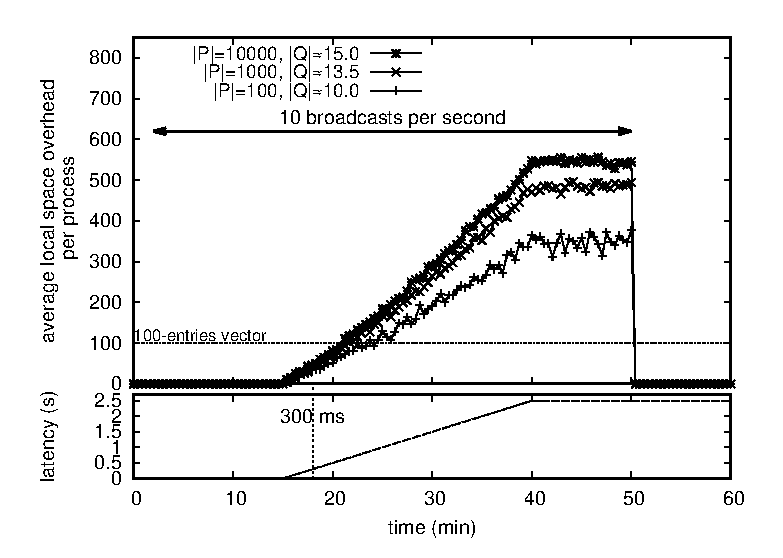
\includegraphics[width=0.8\textwidth]{img/overhead.eps}
  \end{center}

\end{frame}

\begin{frame}{Experiments: Small traffic overhead}
  \begin{center}
    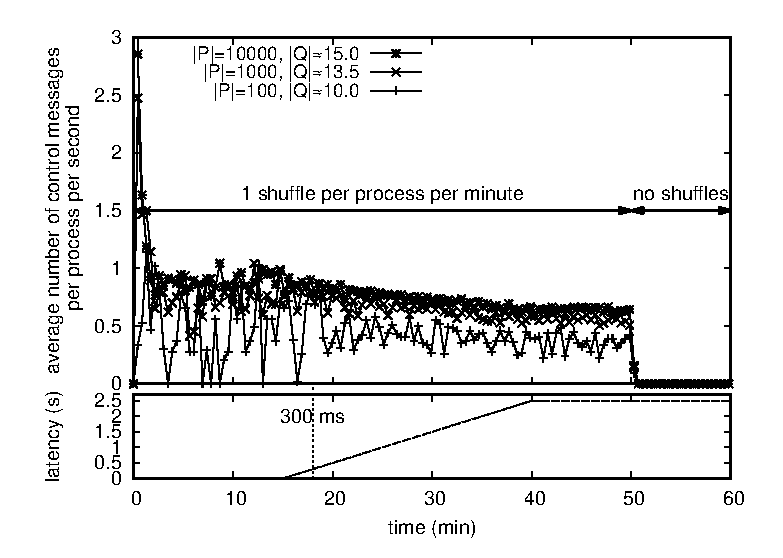
\includegraphics[width=0.8\textwidth]{img/controlmessages.eps}
  \end{center}
\end{frame}


\begin{frame}{Conclusion}
\end{frame}

\begin{frame}[standout]
  To be continued\ldots Retrieving partial order out of flattened orders.
\end{frame}


\end{document}
